\section{Diskussion}
\label{sec:Diskussion}

% Kurze Zusammenfassung der Ergebnisse
% -Vergleich mit Literaturwerten
% -Vergleich mit verschiedenen Messverfahren
% -bei Abweichungen mögliche Ursachen finden

Die durchgeführten Messungen ergeben die innere und gesamte Verdampfungswärme
\begin{align*}
    L_\text{i} =& \SI{0.300+-0.002}{\electronvolt} \\
    L =& \SI{32083+-192}{\joule\per\mol}.
\end{align*}

Ein Referenzwert für die Verdampfungswärme von Wasser bei $T = \SI{100}{\celsius}$ stellt
\begin{equation*}
    L_\text{Referenz} = \SI{40650}{\joule\per\mol}
\end{equation*}
dar. \cite{Verdampfungswaerme}
Also ergibt sich eine Abweichung von
\begin{equation}
    \Delta L = \SI{21.1}{\percent}.
\end{equation}

Diese Abweichung lässt sich durch eine ungenaue Messaperatur und äußere Einflüsse auf den Versuch erklären. 
Außerdem wurden bei der Herleitung der Gleichungen Annahmen getroffen, welche eventuell nicht ganz der Realität entsprechen.

Zu $L_\text{i}$ lässt sich leider kein Vergleichswert finden und kann daher auch nicht näher untersucht werden.

\begin{figure}
    \centering
    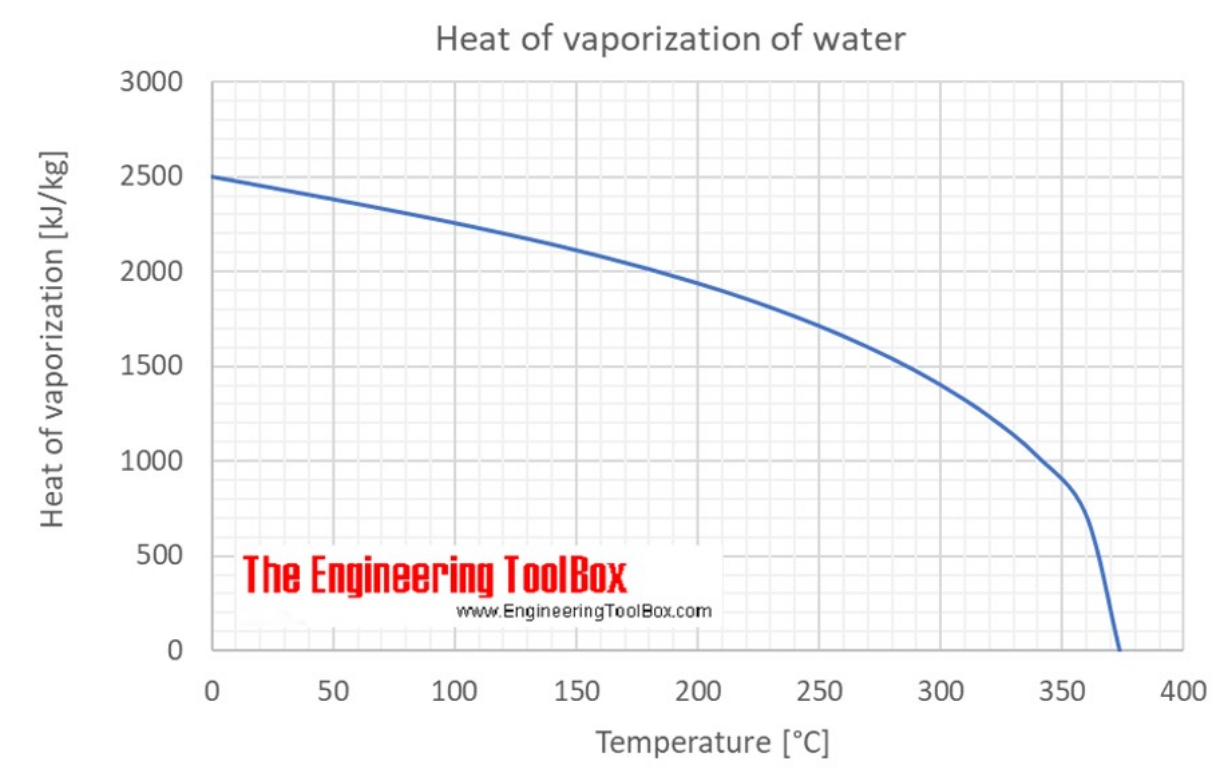
\includegraphics[width=\textwidth]{images/referenz.png}
    \caption{Referenzplot der Temperaturabhängigkeit der Verdampfungswärme. \cite{Verdampfungswaerme}}
    \label{fig:referenz_plot}
\end{figure}

Bei der Temperaturabhängigkeit der Verdampfungswärme lässt sich mit Vergleich zu \autoref{fig:referenz_plot} festellen, dass die Lösung mit $V_{\text{D},+}$ sinnvoller ist, da so, wie in \autoref{fig:plot_hochdruck_plus} gezeigt, die Kurve fällt und nicht steigt.
Eine genauere Diskussion dieser Kurve ist allerdings nicht möglich, da hierfür der Referenzplot eine zu große Skala aufweist.
